% Defence slides (Beamer) — distilled from the validated thesis.
% Reuses validated figures via graphicspath; numbers match the thesis (Phases D/E).
% English (matches the EN-GB thesis); the PT-PT single study source is slides/guia_estudo/main.pdf.
\documentclass[aspectratio=169]{beamer}
\usetheme{Madrid}
\usecolortheme{seahorse}
\usepackage[T1]{fontenc}
\usepackage{booktabs}
\usepackage{tikz}
\usetikzlibrary{positioning, arrows.meta, calc}
% Nos diagramas, nunca cortar palavras a meio (quebrar so em espacos).
\tikzset{every node/.append style={execute at begin node={\hyphenpenalty=10000\exhyphenpenalty=10000\relax}}}
\graphicspath{{../thesis/figures/}}
\setbeamertemplate{navigation symbols}{}
\setbeamertemplate{caption}{\raggedright\insertcaption\par}

\title[InvestiGator]{Explainable Financial Alerts for Retail Investors}
\subtitle{Integrating Statistical Anomaly Detection and News--Market Impact Correlation}
\author[H.\ Santos]{Henrique J.\ S.\ Santos \\ \footnotesize Advisor: Prof.\ Lu\'is Gomes \quad Co-advisor: Rafael Silva}
\institute[ISEP]{MEIA, Instituto Superior de Engenharia do Porto}
\date{\footnotesize Defence}

\begin{document}

\begin{frame}\titlepage\end{frame}

\begin{frame}{The problem}
\begin{columns}
\column{0.58\textwidth}
\begin{itemize}
  \item Most Americans own stock; many now trade through commission-free apps.
  \item The US equity market reached \textbf{US\$62.2\,trillion} (end 2024).
  \item Retail investors face \emph{continuous} price moves and news, \textbf{without} the tools of banks and funds.
  \item The AI spreading through finance is largely \textbf{opaque}, a poor fit for someone who must act and live with the result.
\end{itemize}
\column{0.42\textwidth}
\begin{block}{The three questions}
\small
When a holding moves, everyone asks the same three:
\begin{enumerate}
  \item Is this \emph{unusual for this stock}?
  \item Is it the \emph{company}, or the market?
  \item Has this \emph{happened before}, and what followed?
\end{enumerate}
\end{block}
\end{columns}
\vfill
{\small Free tools answer \textbf{none} of the three; they report the percentage, which is where
question~1 \emph{starts}. A Bloomberg terminal answers all three, for about \$2{,}000 a month.
The gap is not data, which is abundant and free. It is \textbf{context you can check}.}
\end{frame}

\begin{frame}{What InvestiGator does (and does not do)}
\begin{block}{It does \emph{not} predict prices. It \textbf{explains}.}
For each abrupt move or relevant news item, it shows \emph{what} was detected, \emph{how}, the \emph{sources}, and which \emph{past events} resemble it, with what happened to prices afterwards.
\end{block}
\centering
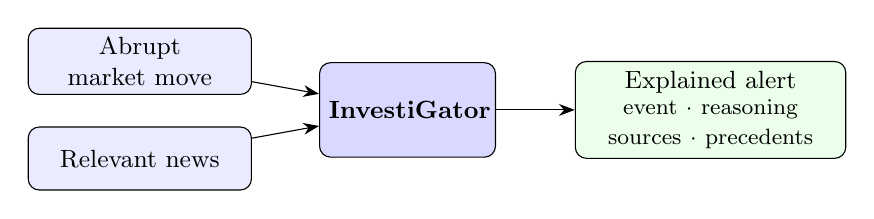
\begin{tikzpicture}[font=\small, >={Stealth[length=2mm]},
  trig/.style={draw, rounded corners, fill=blue!8, align=center, text width=2.6cm, minimum height=0.8cm},
  sys/.style={draw, rounded corners, fill=blue!15, align=center, text width=2.0cm, minimum height=1.2cm},
  outbox/.style={draw, rounded corners, fill=green!8, align=center, text width=3.2cm, minimum height=1.2cm}]
  \node[trig] (t1) {Abrupt market move};
  \node[trig, below=4mm of t1] (t2) {Relevant news};
  \node[sys] (s) at ($(t1)!0.5!(t2)+(3.4,0)$) {\textbf{InvestiGator}};
  \node[outbox, right=1.0cm of s] (o) {Explained alert\\ \footnotesize event $\cdot$ reasoning\\ \footnotesize sources $\cdot$ precedents};
  \draw[->] (t1)--(s); \draw[->] (t2)--(s); \draw[->] (s)--(o);
\end{tikzpicture}
\end{frame}

\begin{frame}{Research questions}
\begin{enumerate}
  \item[\textbf{RQ1}] Can \textbf{transparent} statistical methods detect abrupt moves consistently enough to be useful, while staying explainable?
  \item[\textbf{RQ2}] Can a news--market engine retrieve \textbf{genuinely analogous} precedents and quantify their impact \textbf{without lookahead}, better than trivial baselines?
  \item[\textbf{RQ3}] Can the explanations be \textbf{faithful} to what the system computes, and useful to a retail investor?
  \item[\textbf{RQ4}] Can a \textbf{supervised model}, trained on historical news and market context, usefully \textbf{prioritise} which news deserve an alert, beyond volatility baselines --- \textbf{never} predicting direction?
\end{enumerate}
\vfill
\begin{block}{Contribution: Artificial Intelligence \emph{Engineering}}
Not a new algorithm: the \textbf{disciplined integration, application and critical evaluation} of existing components --- plus \textbf{one model trained by the author} (materiality triage) --- into a working, explainable, reproducible system.
\end{block}
\end{frame}

\begin{frame}{Architecture}
\centering
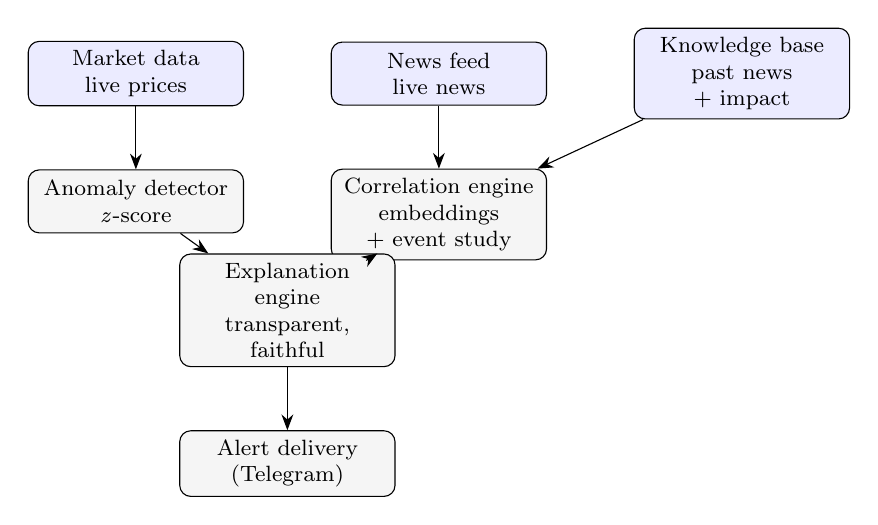
\begin{tikzpicture}[font=\footnotesize, >={Stealth[length=2mm]}, node distance=0.8cm and 1.1cm,
  srcbox/.style={draw, rounded corners, fill=blue!8, align=center, text width=2.5cm, minimum height=0.8cm},
  comp/.style={draw, rounded corners, fill=gray!8, align=center, text width=2.5cm, minimum height=0.8cm}]
  \node[srcbox] (md) {Market data\\ \footnotesize live prices};
  \node[srcbox, right=of md] (nf) {News feed\\ \footnotesize live news};
  \node[srcbox, right=of nf] (kb) {Knowledge base\\ \footnotesize past news + impact};
  \node[comp, below=of md] (an) {Anomaly detector\\ \footnotesize \emph{z}-score};
  \node[comp, below=of nf] (ce) {Correlation engine\\ \footnotesize embeddings + event study};
  \node[comp] (ex) at ($(an)!0.5!(ce)+(0,-1.3)$) {Explanation engine\\ \footnotesize transparent, faithful};
  \node[comp, below=0.8cm of ex] (tg) {Alert delivery (Telegram)};
  \draw[->] (md)--(an); \draw[->] (nf)--(ce); \draw[->] (kb)--(ce);
  \draw[->] (an)--(ex); \draw[->] (ce)--(ex); \draw[->] (ex)--(tg);
\end{tikzpicture}
\par\vspace{2mm}
\footnotesize Single-responsibility components, common schema; two triggers converge on one explanation step.
\end{frame}

\begin{frame}{The data model --- the objects}
\centering
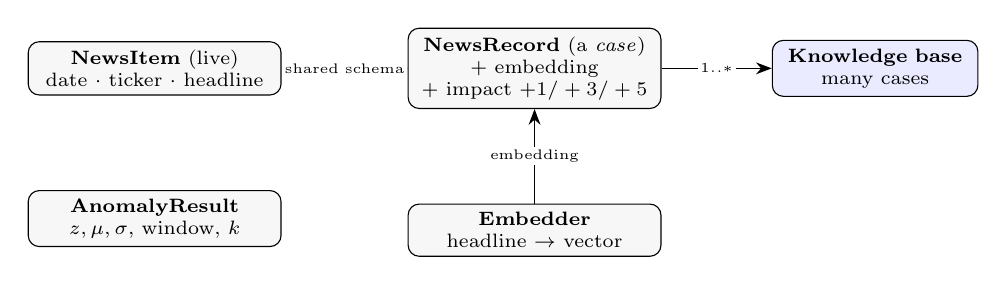
\begin{tikzpicture}[font=\scriptsize, >={Stealth[length=2mm]},
  e/.style={draw, rounded corners, fill=gray!6, align=center, text width=3.0cm, inner sep=3pt},
  st/.style={draw, rounded corners, fill=blue!8, align=center, text width=2.4cm, inner sep=3pt},
  lbl/.style={midway, font=\tiny, fill=white, inner sep=1pt}]
  \node[e]  (ni) {\textbf{NewsItem} (live)\\ date $\cdot$ ticker $\cdot$ headline};
  \node[e, right=1.6cm of ni] (nr) {\textbf{NewsRecord} (a \emph{case})\\ $+$ embedding\\ $+$ impact $+1/+3/+5$};
  \node[st, right=1.4cm of nr] (kb) {\textbf{Knowledge base}\\ many cases};
  \node[e, below=1.2cm of nr] (emb) {\textbf{Embedder}\\ headline $\to$ vector};
  \node[e, below=1.2cm of ni] (ar) {\textbf{AnomalyResult}\\ \scriptsize $z,\mu,\sigma$, window, $k$};
  \draw[->] (ni) -- node[lbl]{shared schema} (nr);
  \draw[->] (nr) -- node[lbl]{$1..*$} (kb);
  \draw[->] (emb) -- node[lbl]{embedding} (nr);
\end{tikzpicture}
\par\vspace{2mm}
\footnotesize A \emph{case} $=$ one past headline $+$ what happened to its price. Live \textbf{NewsItem} and
historical \textbf{NewsRecord} share the schema, so a new headline is directly comparable.
\end{frame}

\begin{frame}{The data, at every stage --- one real headline}
\centering
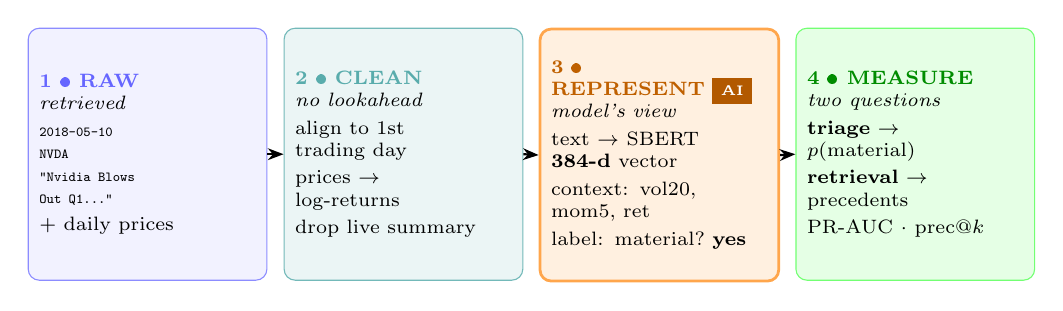
\begin{tikzpicture}[font=\scriptsize, >={Stealth[length=2mm]},
  stage/.style={draw, rounded corners, align=left, text width=2.75cm, inner sep=4pt,
                minimum height=3.2cm, anchor=north},
  raw/.style={stage, fill=blue!5, draw=blue!45},
  clean/.style={stage, fill=teal!8, draw=teal!55},
  rep/.style={stage, fill=orange!12, draw=orange!70, line width=1pt},
  learn/.style={stage, fill=green!10, draw=green!55}]
  \node[raw] (s1) at (0,0){%
    \textcolor{blue!60}{\textbf{1 \textbullet\ RAW}}\\ \emph{retrieved}\\[2pt]
    {\tiny\ttfamily 2018-05-10}\\ {\tiny\ttfamily NVDA}\\ {\tiny\ttfamily "Nvidia Blows}\\ {\tiny\ttfamily Out Q1..."}\\[2pt]
    $+$ daily prices};
  \node[clean] (s2) at (3.25,0){%
    \textcolor{teal!65}{\textbf{2 \textbullet\ CLEAN}}\\ \emph{no lookahead}\\[2pt]
    align to 1st\\ trading day\\[2pt]
    prices $\to$\\ log-returns\\[2pt]
    drop live summary};
  \node[rep] (s3) at (6.5,0){%
    \textcolor{orange!75!black}{\textbf{3 \textbullet\ REPRESENT}}~\colorbox{orange!70!black}{\textcolor{white}{\tiny\bfseries AI}}\\ \emph{model's view}\\[2pt]
    text $\to$ SBERT\\ \textbf{384-d} vector\\[2pt]
    context: vol20,\\ mom5, ret\\[2pt]
    label: material?\ \textbf{yes}};
  \node[learn] (s4) at (9.75,0){%
    \textcolor{green!55!black}{\textbf{4 \textbullet\ MEASURE}}\\ \emph{two questions}\\[2pt]
    \textbf{triage} $\to$\\ $p$(material)\\[2pt]
    \textbf{retrieval} $\to$\\ precedents\\[2pt]
    PR-AUC $\cdot$ prec@$k$};
  \draw[->,thick] (s1.east)--(s2.west);
  \draw[->,thick] (s2.east)--(s3.west);
  \draw[->,thick] (s3.east)--(s4.west);
\end{tikzpicture}
\par\vspace{1mm}
\footnotesize Every value is genuine (Nvidia, 10 May 2018). The ``AI'' is the \textbf{REPRESENT} step:
text becomes a $384$-dimensional embedding, the event becomes context features, the outcome becomes a label.
\end{frame}

\begin{frame}{Market trigger: transparent by design}
\begin{columns}
\column{0.5\textwidth}
Rolling \emph{z}-score, no lookahead:
\[ z_t=\frac{r_t-\mu_t}{\sigma_t},\quad \text{flag if } |z_t|>k \]
$\mu_t,\sigma_t$ over the window \emph{before} $t$. Every quantity is exposed to the explanation.
\column{0.5\textwidth}
\begin{block}{Worked example (real)}
\small TSLA, 24 Oct 2024 (post-earnings):\\
$\mu=-0.92\%$, $\sigma=2.73\%$, $r=+19.8\%$\\
$\Rightarrow z=\mathbf{+7.61}$ (flagged at $k=3$).
\end{block}
A fixed \% threshold would treat a calm and a volatile stock alike; the \emph{z}-score does not.
\end{columns}
\end{frame}

\begin{frame}{Question 2: is it the company, or the market?}
\begin{columns}
\column{0.46\textwidth}
\small
A two-factor market model, estimated \textbf{only on data before the day being explained}:
\[ r_t = \alpha + \beta_m r^{m}_t + \beta_s \tilde r^{\,s}_t + \varepsilon_t \]
The sector factor is \textbf{orthogonalised} against the market (an ETF and the index are
collinear; without it the attribution is meaningless).
\medskip

Betas are \textbf{shrunk by precision}, not clipped: a noisy 20-day estimate is pulled toward its
prior, a clean one is left alone.
\column{0.54\textwidth}
\begin{block}{Real, from the live system}
\small
\textbf{AMZN $-1.84\%$ today} \\[2pt]
$= -1.66\%$ market $\cdot$ $-0.37\%$ sector $\cdot$ $\mathbf{+0.19\%}$ \textbf{company} \\[3pt]
\emph{``Moved with the whole market.''}
\end{block}
{\small The stock fell almost two percent and the company's own contribution was
\textbf{positive}. For the long-term holder, the most valuable output a system can give is often
\textbf{permission to ignore something}.}
\medskip

{\footnotesize Components sum to the observed move by construction, so the line cannot lie.}
\end{columns}
\end{frame}

\begin{frame}{News trigger: retrieve analogous precedents, measure impact}
\begin{columns}
\column{0.52\textwidth}
\begin{enumerate}\small
  \item Embed the headline (Sentence-BERT).
  \item Cosine similarity vs the knowledge base.
  \item Return top-$k$ precedents.
  \item Measure their impact at $+1/+3/+5$ days, from the event-day close (\textbf{no lookahead}).
\end{enumerate}
\emph{Case-based reasoning}: evidence, not a forecast.
\column{0.48\textwidth}
\begin{block}{Worked example (real)}
\scriptsize Query: ``Nvidia demand surges on AI chip orders''\\[2pt]
$\to$ NVDA guidance (sim 0.60) +5d $+3.5\%$\\
$\to$ MSFT cloud-AI (sim 0.38) +5d $+10.9\%$\\
$\to$ NVDA accelerator (sim 0.38) +5d $+4.9\%$\\[2pt]
\textbf{Cross-ticker} match (MSFT); mean +5d $\approx +6.5\%$.
\end{block}
\end{columns}
\end{frame}

\begin{frame}{Result 1: anomaly detection is consistent across the market}
\begin{columns}
\column{0.54\textwidth}
\centering
\includegraphics[width=\linewidth]{eval_anomaly_firing_rate.pdf}
\column{0.46\textwidth}
\begin{itemize}\small
  \item Firing-rate range across 15 tickers: \textbf{0.015} (\emph{z}-score) vs \textbf{0.344} (fixed \%).
  \item $>20\times$ more consistent, a \textbf{label-free} argument.
  \item Vs extreme-move proxy: $F_1=\mathbf{0.516}$ vs $0.218$.
  \item Window ablation: $F_1$ 0.385 / 0.516 / 0.678 (10/20/60 d).
\end{itemize}
\end{columns}
\end{frame}

\begin{frame}{Result 2: semantic retrieval beats every baseline}
\begin{columns}
\column{0.5\textwidth}
\centering
\scriptsize
\begin{tabular}{lcc}
\toprule
Method & P@5 & P@10 \\
\midrule
SBERT (MiniLM) & $0.514$ & $0.478$ \\
SBERT (MPNet) & $\mathbf{0.538}$ & $\mathbf{0.506}$ \\
Lexical & $0.346$ & $0.314$ \\
Recency & $0.126$ & $0.106$ \\
Random & $0.240$ & $0.240$ \\
\bottomrule
\end{tabular}
\par\vspace{1mm}
\scriptsize Cross-ticker, 3{,}714 headlines, 5 seeds ($\pm\sim0.01$).
\column{0.5\textwidth}
\centering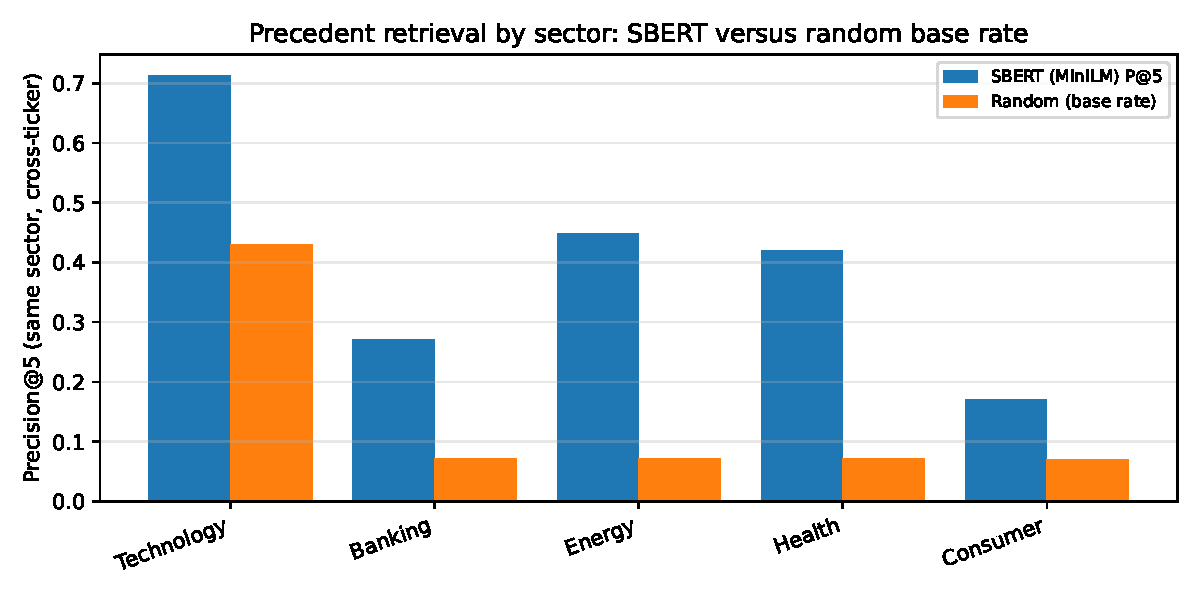
\includegraphics[width=\linewidth]{eval_retrieval_per_sector.pdf}
\par\scriptsize Lift largest where vocabulary is distinctive (energy, health).
\end{columns}
\vspace{1mm}\par\centering\footnotesize Validated at scale on multi-year FNSPID (${\sim}80$k headlines): \textbf{P@5 $0.595$}; direction consistency $0.71$ sits at the $0.69$ chance floor (theme, not direction).
\end{frame}

\begin{frame}{Result 3: explanations are faithful by construction}
\begin{columns}
\column{0.52\textwidth}
\begin{itemize}\small
  \item Each alert is rendered \emph{directly} from the computed objects.
  \item So the text \textbf{cannot diverge} from the computation.
  \item Checked by an automated test (alert reproduces each precedent's date/ticker/impact).
  \item Every alert ends with a no-prediction disclaimer.
\end{itemize}
\column{0.48\textwidth}
\begin{block}{\scriptsize Real alert (news trigger)}
\tiny\ttfamily
News alert --- NVDA\\
``Nvidia raises guidance\ldots AI data-centre''\\
Avg 1-day move: $-1.97\%$ (over 5; 3 shown)\\
- MSFT (0.68) +1d $-3.46\%$\\
- META (0.68) +1d $-2.65\%$\\
- GOOGL (0.64) +1d $-0.46\%$\\
\emph{observed past outcome, not a prediction}
\end{block}
\end{columns}
\end{frame}

\begin{frame}{Result 3b: the same guarantee, for generated language}
\begin{columns}
\column{0.52\textwidth}
\small
A language model was added \textbf{strictly as a narrator}: it may phrase the evidence, never
supply it. A guard validates every response before delivery and \textbf{discards the whole thing} on:
\begin{itemize}\small
  \item a number absent from the evidence,
  \item a figure whose \textbf{sign} was inverted,
  \item predictive or advisory wording,
  \item an attribution contradicting the computed one.
\end{itemize}
The guarantee is a property of \textbf{the system}, not of the model behaving well.
\column{0.48\textwidth}
\begin{block}{Two numbers, deliberately}
\small
\textbf{Pre-guard:} the raw model violated the evidence in a few cases.\\
\emph{$\Rightarrow$ why the guard exists.}\\[4pt]
\textbf{Delivered:} \textbf{zero} violations.\\
\emph{$\Rightarrow$ the guard is what is on trial.}
\end{block}
{\footnotesize\textbf{Honest caveat:} the second is partly circular, since the same checker
decides and grades. The counterweight is a red-team corpus: an independent exercise broke the
\emph{first} design (a blocklist) with 29 reproduced bypasses. Paraphrase space is unbounded and
any list of it is finite, so the guard was rebuilt as a \textbf{closed vocabulary}. Those attacks
are now permanent regression tests.}
\end{columns}
\end{frame}

\begin{frame}{Result 4: learned triage --- trained, calibrated, honest}
\begin{columns}
\column{0.55\textwidth}
\begin{itemize}\small
  \item \textbf{Task:} $P(\text{abnormal move follows news})$ --- materiality, \textbf{never} direction. Labels from our own event study ($|$ticker $-$ SPY$| \ge 2\%$ over $(d,d{+}3]$).
  \item \textbf{Corpus:} FNSPID 2018--2023, $79{,}753$ examples; temporal split by day + embargo; calibration on validation only.
  \item \textbf{Anti-lookahead:} a unit test \emph{mutates future prices} --- features unchanged, label changes.
\end{itemize}
\column{0.45\textwidth}
\scriptsize
\begin{tabular}{l c c}
\toprule
Model & PR-AUC & P@5/day \\
\midrule
Always (floor) & 0.378 & 0.163 \\
\textbf{Volatility LR} & \textbf{0.542} & \textbf{0.632} \\
Context LR & 0.538 & 0.632 \\
Context$+$text LR & 0.496 & 0.585 \\
Gradient boosting & 0.469 & 0.551 \\
\bottomrule
\end{tabular}
\end{columns}
\vfill
\begin{block}{\small The honest verdict (pre-committed)}
\small Within a 5-alerts/day budget, triage nearly \textbf{quadruples precision} ($0.632$ vs $0.163$) --- but \textbf{no text model beat volatility}. A follow-up ablation added \emph{five} more cheap context features (market regime, momentum, standardised reaction, downside risk): PR-AUC $0.535$, again \textbf{no gain}. A \emph{fair} re-test (tuned $C$, PCA-reduced text, a FinBERT domain encoder) still never beat volatility, so the negative is \textbf{robust}, not an under-fit artefact. The signal is market context; reported as it fell.
\end{block}
\end{frame}

\begin{frame}{Result 5: what the system does \emph{not} know}
\small Four studies that examine the system from outside. Each ends in a decision \textbf{not} to
change production, taken on the evidence. The fourth, multi-signal convergence, adapted from
\textbf{worldmonitor.app} on the co-supervisor's recommendation: fusing four independent signals
beat the best single one at \emph{one} alert budget out of three, so it stays a measurement. Its
by-product, a \textbf{volume} detector at zero data cost, is kept.
\vspace{1mm}
\begin{columns}[T]
\column{0.33\textwidth}
\textbf{\footnotesize Event types}\par\smallskip
{\scriptsize Clustered the embeddings against a rubric written \emph{before} clustering.
Agreement (chance-corrected): event \textbf{0.358} $>$ ticker $0.188$ $>$ sector $0.130$.
\par\smallskip
So the space \emph{does} encode event type, more than subject. But separation is weak
($\text{silhouette }0.084$) $\Rightarrow$ \textbf{not} wired to retrieval: a wrong event type drops
valid precedents silently.}

\column{0.33\textwidth}
\textbf{\footnotesize Conformal guarantee}\par\smallskip
{\scriptsize Distribution-free coverage on the \emph{frozen} model (PR-AUC reproduced exactly first).
\par\smallskip
Holds at 90\%/80\%; \textbf{breaks at 95\%} under a temporal split. Tighter coverage leans on the
tail, and the tail moves first.
\par\smallskip
\textbf{The price:} to promise 90\%, a definite call on only \textbf{39.5\%} of headlines.}

\column{0.33\textwidth}
\textbf{\footnotesize Drift, measured}\par\smallskip
{\scriptsize The limitation we kept \emph{asserting}, finally sized.
\par\smallskip
Pre-event volatility PSI \textbf{0.281} (significant); returns features $0.020$ / $0.014$ (stable).
\par\smallskip
Label prevalence \emph{oscillates} ($0.385 \to 0.470 \to 0.378$), it does not trend. Gives a
\textbf{retraining trigger} instead of an intuition.}
\end{columns}
\vfill
\begin{block}{\small Why this matters more than another positive number}
\small The 39.5\% figure \textbf{explains} Result 4 from an independent angle, without training
anything new: the available signal genuinely does not separate most items. And the drift result
tells us \emph{why} the frozen numbers survive, because the protocol already crosses one such
oscillation.
\end{block}
\end{frame}

\begin{frame}{The product, live}
\begin{columns}
\column{0.55\textwidth}

\includegraphics[width=\linewidth]{app_dashboard.png}
\column{0.45\textwidth}
\small
A genuine screenshot, not a mockup. \textbf{Three screens, one per question:}
\begin{itemize}\small
  \item \textbf{Today} --- the watchlist ranked by how far from normal, with the
        market/sector/company split \textbf{on the row}. No click needed.
  \item \textbf{Ticker} --- chart, full decomposition, and the alerts \emph{exactly} as the
        Telegram channel received them. Never recomputed.
  \item \textbf{Method} --- the frozen numbers, including the negative result.
\end{itemize}
{\footnotesize The promise appears \textbf{once}, as the page's identity. The latency figure is
\textbf{measured} and is simply absent when the timestamps are not there.}
\end{columns}
\end{frame}

\newcommand{\techbadge}[2]{{\setlength{\fboxsep}{3pt}\colorbox{#1!13}{\small\strut #2}}}
\newcommand{\techcat}[1]{\smallskip\par\textbf{\footnotesize #1}\par\smallskip}
% Real logo if slides/logos/<file>.png exists; otherwise a clean name-badge (see logos/README.md).
\newcommand{\techlogo}[3]{\IfFileExists{logos/#1.png}%
  {\raisebox{-3pt}{\includegraphics[height=13pt]{logos/#1.png}}~}{}\techbadge{#2}{#3}}
\begin{frame}{Built with --- free tools and open data, end to end}
\centering\vspace{1mm}
\techcat{\textcolor{blue!60}{Data sources \& APIs}}
\techlogo{huggingface}{blue}{FNSPID (Hugging Face)}\ \techlogo{yfinance}{blue}{yfinance}\ %
\techlogo{finnhub}{blue}{Finnhub}\ \techlogo{rss}{blue}{RSS feeds}\ \techbadge{blue}{SPY (market proxy)}
\techcat{\textcolor{orange!75!black}{Machine learning}}
\techlogo{sbert}{orange}{Sentence-BERT / MiniLM}\ \techlogo{scikit-learn}{orange}{scikit-learn}\ %
\techlogo{pytorch}{orange}{PyTorch (CPU)}\ \techbadge{orange}{Platt calibration}\ %
\techlogo{onnx}{orange}{ONNX Runtime}
\techcat{\textcolor{green!55!black}{Product \& delivery}}
\techlogo{telegram}{green}{Telegram Bot API}\ \techlogo{streamlit}{green}{Streamlit}\ %
\techlogo{plotly}{green}{Plotly}
\techcat{\textcolor{purple!70}{Engineering \& infrastructure}}
\techlogo{python}{purple}{Python 3.12}\ \techlogo{githubactions}{purple}{GitHub Actions (cron)}\ %
\techlogo{pytest}{purple}{pytest $+$ ruff}\ \techbadge{purple}{joblib}
\par\bigskip
{\footnotesize No paid APIs, no GPUs, no always-on server --- reproducible on a laptop.}
\end{frame}

\begin{frame}{Limitations (stated plainly)}
\begin{itemize}
  \item Relevance is a \textbf{same-sector proxy}, not a human judgement.
  \item Retrieval corpus is a \textbf{recent} free-tier window (since validated at scale on FNSPID, P@5 $0.595$); the \emph{triage} study did use multi-year FNSPID (14/15 tickers --- Meta is ``FB'' in the corpus).
  \item Displayed precedent impact is a \textbf{raw} post-event return (triage labels \emph{are} market-adjusted).
  \item Similarity is \textbf{thematic, not directional}: a cluster can mix up/down moves, so the mean is theme-level \emph{evidence}, not a forecast. We \emph{tested} the obvious fix (filter by event type) and it does not hold up --- see Result 5.
  \item \textbf{Confidence is thin, and now quantified:} guaranteeing 90\% coverage leaves a definite call on only \textbf{39.5\%} of headlines.
  \item \textbf{Train/deploy drift is measured, not just claimed:} concentrated in volatility (PSI $0.281$), and cyclical rather than trending.
  \item \textbf{No human usefulness study} yet (RQ3 usefulness open).
  \item By design: \textbf{no price prediction, no trading}, so profit metrics are out of scope.
\end{itemize}
\vfill
\footnotesize All results are reproducible from versioned scripts (re-run: identical numbers).
Two of the limitations above used to be assertions; they are now measurements.
\end{frame}

\begin{frame}{Conclusions}
\begin{itemize}
  \item \textbf{RQ1 (yes):} transparent \emph{z}-score detects consistently across the market and explains every flag.
  \item \textbf{RQ2 (yes, validated at scale):} semantic retrieval far above baselines (P@5 $0.595$ on multi-year FNSPID); impact measured without lookahead.
  \item \textbf{RQ3 (faithful yes; useful open):} explanations cannot diverge from the computation; human usefulness is future work.
  \item \textbf{RQ4 (no on text; yes on mechanism):} triage $\approx 4\times$ within-budget precision, but volatility stayed unbeaten --- the \emph{second} fair ``learned vs simple'' test the transparent choice won (first: Isolation Forest vs \emph{z}-score, $F_1$ $0.271$ vs $0.530$).
\end{itemize}
\vfill
\begin{block}{Contribution}
A working, \textbf{explainable, reproducible} financial-alert system for retail investors --- existing components plus one author-trained triage model, engineered into a transparent whole, with an honest evaluation.
\end{block}
\end{frame}

\begin{frame}{Thank you}
\vfill
\centering
{\Huge \textbf{InvestiGator}} \\[4mm]
{\large Explainable financial alerts for retail investors} \\[8mm]
{\footnotesize Questions welcome.}
\vfill
\end{frame}

\begin{frame}{Anticipated questions}
\footnotesize
\begin{itemize}
  \item \textbf{Why not predict prices?} Market efficiency (Fama 1970): public news is impounded fast; we \emph{measure} reactions, honestly.
  \item \textbf{Why \emph{z}-score, not Isolation Forest/GARCH?} Transparency for a low-dimensional signal --- and we \emph{tested} it: a causal Isolation Forest on the same information lost ($F_1$ $0.271$ vs $0.530$).
  \item \textbf{Your trained model lost to the volatility baseline. Failure?} No: the comparison was \emph{pre-committed} and answers RQ4 with evidence; triage still $\approx 4\times$ within-budget precision vs alerting always, and the deployed variant uses exactly the features that carry the signal.
  \item \textbf{How do you know the triage model never sees the future?} A unit test mutates post-event prices and asserts features are unchanged while the label changes; temporal split by unique day with a five-day embargo.
  \item \textbf{Why precision@$k$ and a sector proxy?} Standard ranked-retrieval metric; objective, reproducible; human relevance is future work.
  \item \textbf{Cross-ticker constraint?} An \emph{evaluation} choice to avoid trivial self-matches; the live alert shows the most similar precedents regardless.
  \item \textbf{A positive headline retrieved negative precedents ($-1.97\%$). Misleading?} Similarity matches \emph{theme}, not direction; the mean is theme-level \textbf{evidence}, shown with every precedent and a no-prediction disclaimer. Future work: de-duplicate precedents and flag directional disagreement.
  \item \textbf{Is it reproducible?} Yes: fixed seeds, pinned deps, versioned scripts; re-running reproduces every number.
\end{itemize}
\end{frame}

\begin{frame}{Anticipated questions (continued)}
\footnotesize
\begin{itemize}
  \item \textbf{Isn't ``zero delivered violations'' circular, since your own checker grades it?}
        Partly, and the thesis says so. That is why it is not the only test: an independent
        red team broke the \emph{previous} guard with 29 reproduced bypasses, built without
        sight of the current design, and those attacks are now regression tests.
  \item \textbf{So you built a multi-agent system?} No, and I will not claim it. One model
        calling a few functions is not multi-agent. The narrator is a \textbf{pure function}
        from evidence to a paragraph.
  \item \textbf{Why exclude analyst price targets? They are free.} Because importing someone
        else's forecast into a system defined by not forecasting is a contradiction. Coherence
        was preferred to coverage, and it is stated as a position in Chapter~6.
  \item \textbf{Why no portfolio features?} Holdings are personal financial data, and
        ``your top positions are one bet'' is advice however it is phrased. That crosses the
        boundary the ethical claim depends on.
  \item \textbf{Where does the $0.5$ triage threshold come from?} Originally nowhere, which was
        the honest problem. Sweeping it under an explicit cost ratio showed it implicitly assumed
        a miss costs about the same as a false alarm; under equal costs the optimum sits where
        the constant already was. Vindicated, but now \emph{derived}.
  \item \textbf{Your alerts arrive hours late.} Measured: a median of about three hours, and the
        cause is the free scheduler, not the method. The always-on path is written and costs
        about a minute; deploying it was out of scope for the evaluation, and the honest number
        is displayed in the product rather than hidden.
\end{itemize}
\end{frame}

\end{document}
